\section{Solar System Pipelines}
\label{sec:solsys}

\begin{figure}[th]
\begin{center}
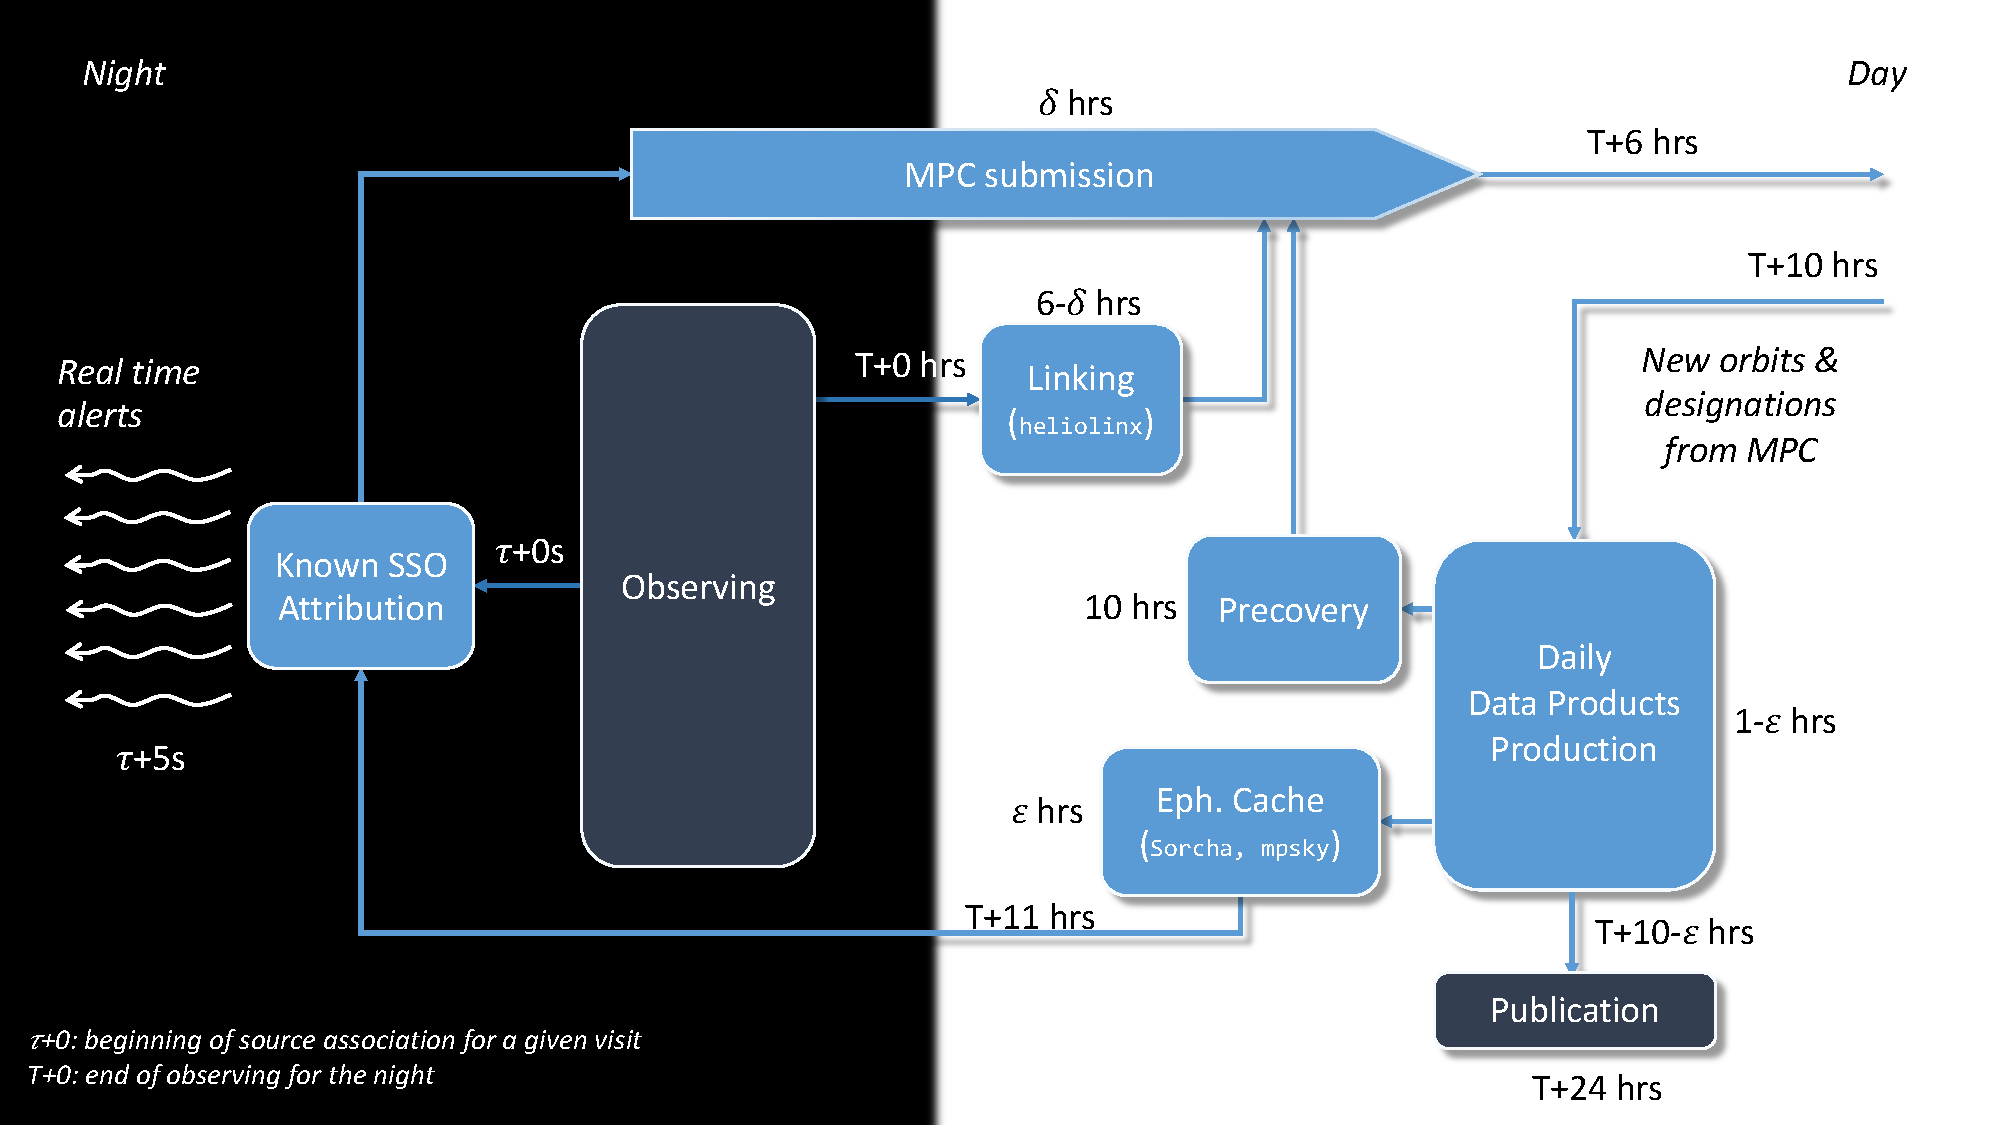
\includegraphics[width=0.45\textwidth]{figures/solarsystempipeline.pdf}

\caption{\label{fig:ssp} Detection, attribution, linking, submission and precovery of moving sources within the nightly data: The attribution is performed in real-time by the AP pipelines querying the {\tt mpsky} service with resulting information attached to the alerts and queued for submission to the MPC.  The linking is performed in daytime using {\tt heliolinx}, with resulting links queued for submission to the MPC.  Fetching of data from the MPC is performed automatically using PostgreSQL replication, with new data triggering recomputation of physical properties and precovery runs in the Daily Data Products Pipeline.  Any observations discovered by the precovery procedure are queued for submission to the MPC, using the submission manager tool.  The ephemeris cache is precomputed at dusk using {\tt Sorcha} and {\tt mpsky}, to enable fast attribution at nighttime.  All timings denote design goals.  }

\end{center}
\end{figure}
The Solar System Pipeline (SSP; Figure~\ref{fig:ssp}) suite is responsible for (i) discovering previously unknown solar system objects by linking together observations (usually DIASources) unattributable to static (non-moving) sources, (ii) reporting these to the Minor Planet Center (MPC), (iii) computing basic physical characteristics such as absolute magnitudes and slope parameters for all asteroids where sufficient data is available, and (iv) using the orbits received from the MPC to associate their apparitions in the DIASource tables (both in real-time and as precovery). 

The core element of the SSP is the linking pipeline, named {\tt heliolinx} \citep{heliolinx}.  This code, run in daytime, clusters newly detected DIAObjects to search for candidate asteroids.  The high-level procedure is to link DIASource detections within a night (when on-sky motion is approximately linear) into {\em tracklets}, to link these tracklets across multiple nights (into tracks) and to fit the tracks with an orbital model to identify those tracks that are consistent with an asteroid orbit.  The Rubin implementation of this software (Heinze et al., in prep.) is based on the HelioLinC algorithm \citep{2018AJ....156..135H}, with the key change being that the clustering is performed not on the sky, but in 3D space.  It is designed to be capable of detecting 95\% of all Solar System objects whose tracklets are observed over three nights within a 15-night window.\footnote{Detailed criteria are specified in the LSST Observatory System Specification (OSS) document {\tt OSS-REQ-0159}}. {\tt heliolinx} is written in C++, but provides a Python API including a Task API.

Candidate discoveries with high degree of certainty, as well as re-observations of already known objects, are reported to the Minor Planet Center (MPC) using the observation submission pipeline.  The astrometric and photometric data are converted to the PSV variant of the Astrometric Data Exchange Standard \citep[ADES;][]{2017DPS....4911214C}, and submitted via a HTTPS POST API provided by the MPC.

Following processing and validation of newly reported candidates, they're added to the MPC's central database.  This database, including the table orbits as well as observations, is replicated using PostgreSQL logical replication.  Following the replication, the Daily Data Products Pipeline recomputes the absolute magnitudes of objects in the SSObject table, as well as some auxiliary per-observation information for individual observations (the SSSource table).

The replicated orbits and computed absolute magnitudes are utilized to predict positions (ephemerides) and magnitudes of solar system objects at subsequent night.  To enable speedy retrieval (on order of 100msec or less) of all objects in a visit, we precompute on-sky locations of all solar system objects, fit Chebyshev polynomials, and build an efficient HEALpix-based index allowing for fast lookup.  These ephemerides are then served to association pipelines described in Section~\ref{sec:solar}.  This element of the pipeline is based on Sorcha (computation; Merritt et al.  accepted) and {\tt mpsky} \citep[fast lookup and serving;][]{mpsky}.  While still being constructed, a similar service is planned for ``precovery'' -- the association of originally missed observations of solar system objects observed earlier in the survey.
\\

Taken together, this suite of pipelines enables Rubin to identify sources consistent with being observations of objects in the solar system (both new and previously known), and makes these data public by reporting their discoveries to the Minor Planet Center and making them available to Rubin users within via the PPDB.
